\placelogofalse
\begin{frame}{Design Goals}
\begin{columns}
  \column{0.48\linewidth}
  \begin{outline}
    \1 Explore data representation 
    \2 Sparse data structures
    \2 Quantized data types
    \1 Decouple data and algorithms
    \1 Differentiable kernels
    \1 Optimize access patterns
    \1 Optimize parallelism
  \end{outline}

  \column{0.48\linewidth}
  \centering
  \begin{center}
  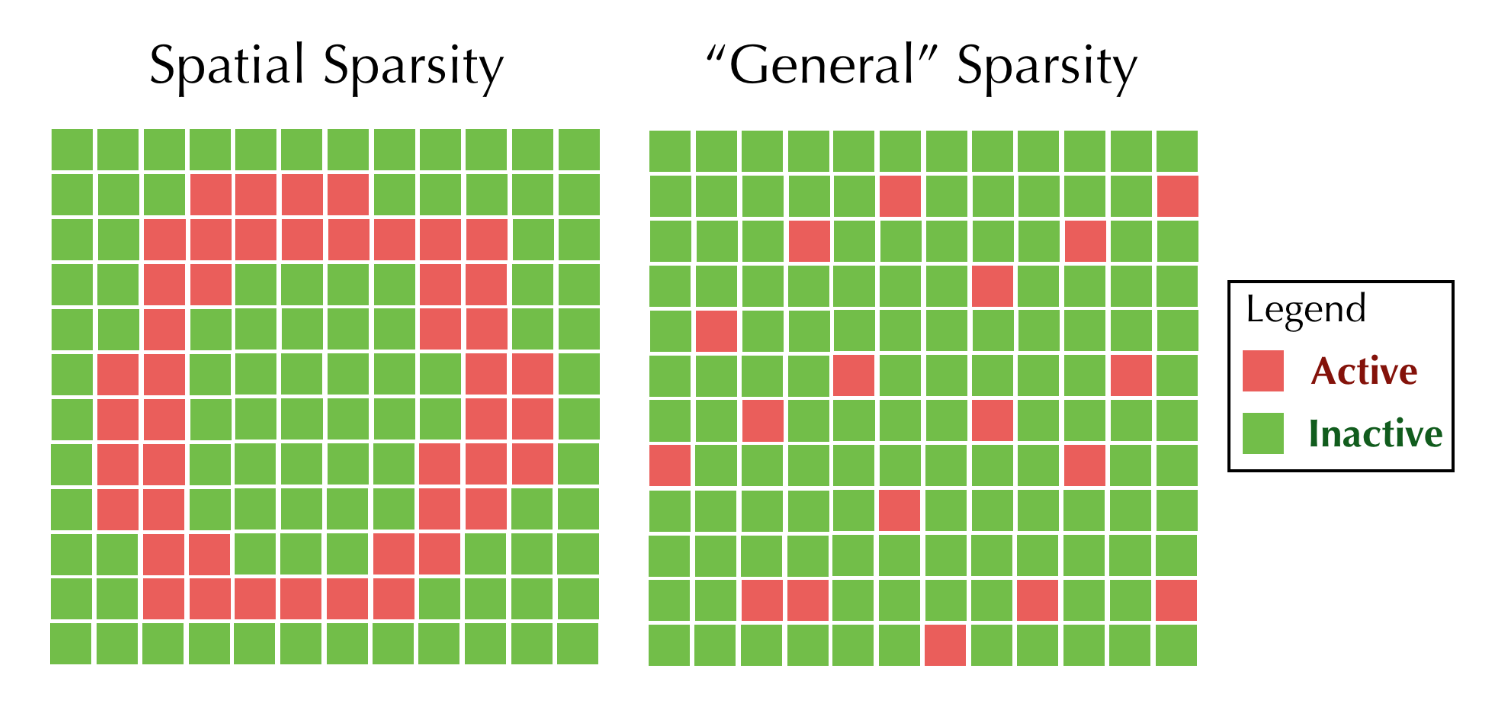
\includegraphics[width=5.0cm]{taichi_sparsity.png}

  \vspace{0.75cm}

  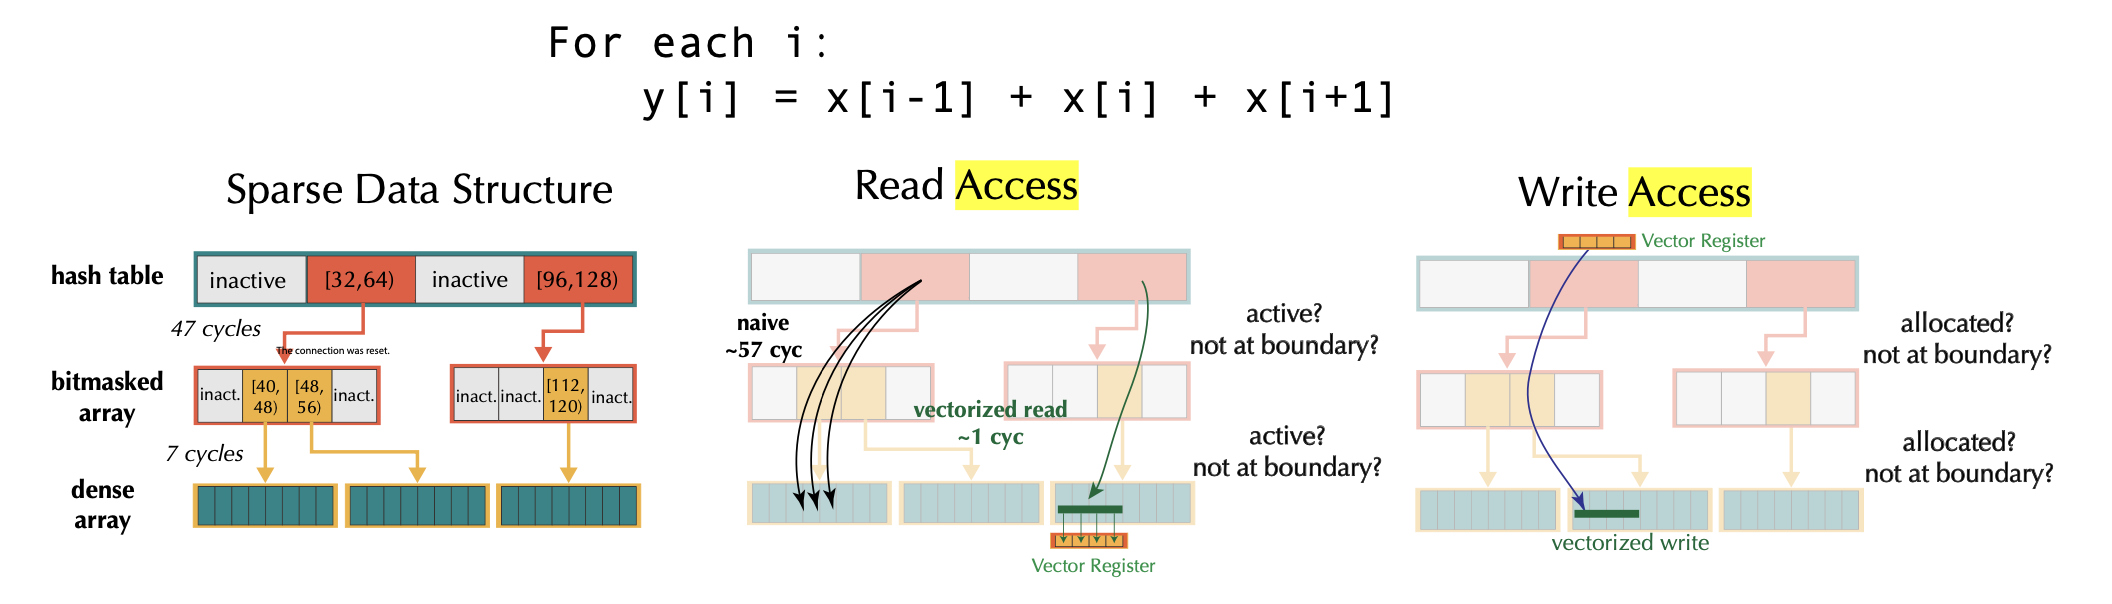
\includegraphics[width=6.0cm]{access_pattern.png}

  \vspace{0.75cm}

  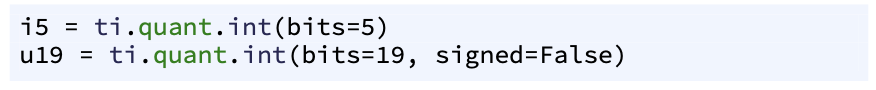
\includegraphics[width=6.0cm]{quantized_types.png}
  \end{center}
\end{columns}
\end{frame}
\placelogotrue
